% !TeX root = ../thuthesis-example.tex

\chapter{绪论}

本文主要针对深度神经网络(Deep Neural Networks)中的重要组件——标准化层(Normalization Layer),设计了一种全新的标准化层结构,并在多种应用场景下,通过大量的分析和实验验证了该结构的效果。

\section{选题背景与意义}
进入二十一世纪以来,伴随着计算机技术的发展和普及,人类对数据的处理和分析能力也迈上了新的台阶。作为数据科学中的极为重要的一环,深度学习则顺应了数据爆炸时代的需求,取得了巨大的发展,越来越多的人开始投身深度学习的研究。
2021年多伦多大学的Alex krizhevsky等人提出AlexNet\citep{krizhevsky2012imagenet},深度学习在图像分类比赛ILSVRC2012中取得了前所未有的好成绩,此前一直处于研究瓶颈的深度学习突然找到了方向,相关研究数量爆炸性的增长,也被逐渐应用到越来越多不同的领域中。近十年里,深度学习在图像处理、计算机视觉、自然语言处理、机器翻译、医学成像、机器人控制等多种任务上都取得了显著的成果。
深度学习,作为机器学习的一个重要分支,相比起传统机器学习而言,最大的优势就在于其强大的表征能力,即从各种类型的输入中提取、生成特征的能力。这一特点使得深度学习的方法能够高效利用大规模的训练数据,也能够在不同任务间进行复用。

\subsection{迁移学习}
迁移学习(Transfer Learning)是机器学习中的一个重要研究问题,其目标是将某个领域或任务上学习到的知识或方法应用到其他不同但是有相关性的领域或问题中。迁移学习的灵感主要来源于人类的学习行为,比如人在学习外语的时候会自发的借助已经掌握的母语知识帮助理解。但是很多问题之间又是很难进行迁移的,比如看似相同的棋类游戏之间往往规则差别很大,熟悉了解某一种棋的技巧可能对另一种没有太大的帮助。
迁移学习相比起传统机器学习最大的优势,便是不在需要训练数据和测试数据服从\textbf{独立同分布}这一假设。迁移学习允许参与学习的领域或任务服从不同的概率分布或条件概率分布,这在很多实际场景中具有很重要的意义,因为在很多实际场景中,为每个领域都收集足够充分的标记数据的代价十分昂贵、甚至无法实现,这在医疗健康、生物信息学等领域十分常见。
而迁移学习的提出以及相关技术的发展,为这些领域的问题提供了一条新的解决途径。

广义的迁移学习一般包括两个数据域,分别记为源域(Source Domain)和目标域(Target Domain),最直接的目标便是利用源域中的知识提升在目标域上学习的效果。图~\ref{fig:transfer}展示了几种实际场景下的迁移学习问题。
迁移学习包含非常多的子分支,分别针对不同的实际场景,例如可以根据源域和目标域是否对训练可见或者是否有标签(Label)等进行分类。其中发展较为迅速的例如领域适应学习(Domain Adaotation)中,
一般源域数据和目标域数据对训练都是可见的,但是目标域的数据不带标签;模型微调(Model Fine-tune)中目标域数据是带有标签的,但是源域数据一般对训练不可见,取而代之的在源域数据上训练得到的知识,比如
神经网络的参数等等;而在领域泛化学习(Domain Generalization)中则只有源域数据对训练可见。不同的子分支任务对源域和目标域知识的利用程度各有不同,因而也有着各自的研究赛道。
但是在深度学习出现以前,迁移学习往往会受限于传统机器学习方法,只能用于解决某些特定的问题。但是随着深度学习逐渐发展,达到现代机器学习中的优势地位,直接扩展了迁移学习的面向领域,为未来迁移学习的发展带来了无限可能。

\begin{figure}
    \centering
    \subcaptionbox{从虚拟路况到真实路况的迁移场景}{
      \includegraphics[width=0.45\linewidth]{figures/绪论/1.jpg}
      \includegraphics[width=0.45\linewidth]{figures/绪论/2.jpg}
    }
    \subcaptionbox{跨仪器设备医疗影像识别}{
      \includegraphics[width=0.52\linewidth]{figures/绪论/ct.png}
      \includegraphics[width=0.46\linewidth]{figures/绪论/核磁.png}
    }
    \caption{迁移学习场景示例}
    \label{fig:transfer}
\end{figure}
    

\subsection{模型微调}

模型微调(Model Fine-tune)是迁移学习中非常重要的子分支之一。这里先对模型微调进行形式化的定义:

\begin{definition}[模型微调]
    假设有一个在源域数据上训练得到的与训练模型$\symup{\Theta}$,以及有$n$条样本的目标域数据集$\mathcal{D}={\{(x_i,y_i)\}_{i=1}^m}$。模型微调的目标是是模型$\symup{\Theta}$在数据集$\mathcal{D}$
    的泛化误差(Generalization Error):
    \begin{equation}
        \mathbb{E}_{(x,y)\sim P_t}[\texttt{Loss}(\symup{\Theta}(x),y)]
    \end{equation}
    最小。
\end{definition}

\begin{figure}
    \centering
    \subcaptionbox{预训练任务}{
        \includegraphics[width=0.9\linewidth]{figures/绪论/pretrain.png}
    }
    \subcaptionbox{模型微调下游任务}{
        \includegraphics[width=0.9\linewidth]{figures/绪论/finetune.png}
    }
    \caption{一些常见的预训练和微调任务}
    \label{fig:finetune}
\end{figure}

由于在模型微调场景下中,深度神经网络一般无法直接获取源域的训练数据,只能利用在这些数据上训练得到的预训练模型,但相应地在模型微调时可以使用到更大规模的训练数据来提升预训练模型的性能,同时也不会额外
增加训练成本。计算机视觉作为深度学习最先获得成功的领域,一定程度上就是因为天然存在大量的图像作为训练数据,但由于研究人员设计的网络结构日渐复杂,在提升深度神经网络效果的同时,也让深度神经网络逐渐变宽变深,
参数量呈指数式暴涨,使得从头训练一个深度神经网络开始变得极其困难。如果依然在大规模的数据上从头开始进行训练,会消耗大量的时间和计算资源,在这一前提下,模型微调成为了具有很重要的实际意义的研究方向。

模型微调的一大特点便是预训练源域数据集和下游目标域数据集的区别。在很多迁移学习场景中,例如领域适应学习和持续学习,源域和目标域数据一般具有相同的规模、相同的内容或者相同的标签,而模型微调则对两者没有
要求。以图像分类的模型微调场景为例,源域数据集一般包含上万张图像数据,涵盖成百上千种大类,具有很强的通用性和泛化性,但是相应地,预训练阶段所需的时间长、资源消耗巨大;而目标域数据集一般规模较小,具有很强的
目的性,一般是针对某种任务进行数据采集,相应地,微调阶段所需的时间短、资源消耗也明显少于预训练阶段。图~\ref{fig:finetune}展示了一些常见的预训练和微调数据集,可以看出预训练数据数目庞大且具有很强的多样性,
而微调数据集则五花八门,差异明显。模型微调这种方式与人类的学习行为也十分类似,人类在面对新事物时并不会直接参考以往全部的相关事物,而是会直接借助以往积累的经验,即“预训练的知识”快速地做出判断。

在很多实际场景下,数据的采集具有很高的代价和风险,基于目标任务采集的数据可能无法保证深度神经网络得到充分地训练,也就无法充分利用深度学习对数据的学习能力。而模型微调则依靠
具有很强通用性和泛化性的预训练模型,在高效利用预训练知识的同时,也很大程度上弥补了下游任务中数据量不足的缺陷,为深度学习的广泛应用创造了无限可能。

\section{研究问题与挑战}

深度学习的发展离不开深度神经网络结构的进步,而无论什么类型的深度神经网络,都离不开标准化层结构。尽管标准化层的设计和算法实现通常比较简单,但是在什么维度进行标准化、如何标准化、为什么要进行标准化等问题,
关系着最终网络性能能否提升。研究人员针对各种任务场景,设计了特有的标准化层结构,从结构层面提高了深度神经网络的性能,取得了非常显著的成果。但是这些结构往往依据该场景下的一些先验假设,
在其他场景中可能不会有效,甚至带来负效应。

利用预训练模型进行模型微调,作为深度学习中使用非常广泛的方法,在许多实际应用场景下都取得了很好的效果。然而目前针对模型微调场景的标准化层结构研究还较为欠缺,研究人员往往选择继承预训练模型使用
的标准化层而不作任何修改。尽管大部分情况下这种方式不会带了负面影响,但是依然忽视了很多模型微调中特有的问题,存在着很大的改进空间。因此,本文选择模型微调场
景下的标准化层为研究课题,旨在分析模型微调场景下现有标准化方法的不足,并针对性地设计全新的标准化层结构,提升模型微调算法的效果。

\section{研究现状}

本节对模型微调以及标准化层领域的相关工作进行简要地概括,在下一章中会进行更加详细的介绍。

\subsection{模型微调}

模型微调领域下根据研究阶段的不同分为预训练阶段和微调阶段。预训练阶段的主要研究问题为如何设计具有更好通用性和泛化性的预训练模型,包括但不限于更大的预训练数据集、更复杂的深度神经网络、更强的预训练技术等等。
一部分数据科学家们会耗时数年构建一个非常庞大的预训练数据集~\citep{deng2009imagenet,sun2017revisiting},而一部分研究工作则针对设计更宽更深的深度神经网络结构~\citep{szegedy_going_2015,szegedy2016rethinking,
he2016deep,huang_densely_2017}。另外一些工作则在前两者的基础上,通过设计新的预训练方式来获得更强的预训练模型,使用诸如掩码模型(Masked Modeling)~\citep{devlin2019bert,bao2021beit,he2021masked}、
对比学习(Contrastive Learning)~\citep{he2020momentum,chen_simple_2020}、提示学习(Prompt Learning)~\citep{liu2021pre,radford2021learning}等方法,进一步挖掘预训练模型的潜力。

而在微调阶段,则更关注于如何基于下游任务的特性,最大程度地利用预训练模型中的知识。在微调阶段,最为常见的研究问题便是灾难性遗忘(Catastrophic Forgetting),会使得深度神经网络在学习下游任务知识的
同时,逐渐丢失预训练模型中的知识,这与模型微调的初衷相悖。因此有很大一部分研究工作针对这一问题,使用基于正则化约束的方法来避免对预训练模型知识的遗忘~\citep{li2017learning,li2018delta,li2018learning,you2020co}。
而有些工作则着眼于不同预训练模型对微调任务的影响,Kornblith等人的工作~\citep{kornblith2018better}通过使用不同深度神经网络结构的预训练模型在不同的下游任务上进行微调,得出了一系列预训练模型对微调影响的结论。
基于这一发现,一些工作提出了对不同的预训练模型进行评判的准则,先选出最适合当前下游任务的预训练模型再进行微调~\citep{tran2019transferability,bao2019information,you2021logme}。也有一些研究人员认为,并不需要
对预训练模型进行筛选,直接对多个预训练模型的特征或者参数进行集成能更大程度上利用预训练的知识~\citep{rusu2016progressive,liu2019knowledge,shu2021zoo}。


\subsection{标准化层}

如今深度学习的迅速发展离不开深度神经网络结构的改进,从最早的多层感知机(Multi-Layer Perceptron,MLP)到卷积神经网络(Convolutional Neural Networks,CNN)和循环神经
网络(Recurrent Neural Networks,RNN),再到目前最为引人注意的Transformer,深度神经网络的每一次迭代,都在各类深度学习任务上取得了标志性的提升。
但是纵观这些风格各异的深度神经网络,在网络规模变大的同时,都离不开一个重要的组件——标准化层。例如多层感知机和卷积神经网络中的批标准化(Batch Normalization)~\citep{ioffe2015BN},循环神经
网络和Transformer中的层标准化(Layer Normalization)\citep{lei2016LayerNorm}等等。

标准化最早是统计学中的概念,一般指参照某一个统一的标准来调整两组数据的构成,从而使其能够互相比较。最常见的标准化便是对一组数据${\{x_i\}}_{i=1}^n$,先计算它们的
均值和方差:
\begin{equation}
\begin{aligned}
    \mu=\frac{1}{n}\sum_{i=1}^n{x_i},\quad
    \sigma^2=\frac{1}{n}\sum_{i=1}^{n}{(x_i-\mu)^2}
\end{aligned}
\end{equation}

再将整组数据减去均值除以方差:

\begin{equation}
    x'=\frac{x-\mu}{\sigma}
\end{equation}

从而使得这组数据的均值为$0$而方差为$1$。

深度学习中对标准化的利用非常丰富,实际场景下主要根据任务的不同,可以在不同的维度上计算特征的均值$\mu$和方差$\sigma$~\citep{ioffe2015BN,lei2016LayerNorm,ulyanov_instance_2016,wu2018GroupNorm},
或者对特征之外的数据,诸如网络参数或者特征的奇异值等进行标准化~\citep{Salimans2016Weight,miyato_spectral_2018}。正是由于标准化技术的多样性,不同的标准化层在不同任务中的效果往往差别很大,
研究人员需要根据实际场景选择或者设计更合适的标准化层结构。

\section{研究内容与主要创新点}

图~\ref{fig:research}为本文的研究框架图。本文主要通过研究深度神经网络结果,设计了一种全新的标准化层,从而提升网络的整体性能,接着在学术界使用的细粒度分类任务上进行了实验,并在实际场
景中的医疗影像任务和风速预测任务进一步验证了其效果,最后借助迁移学习算法库的平台对该标准化层结构进行了集成。

\begin{figure}
    \centering
    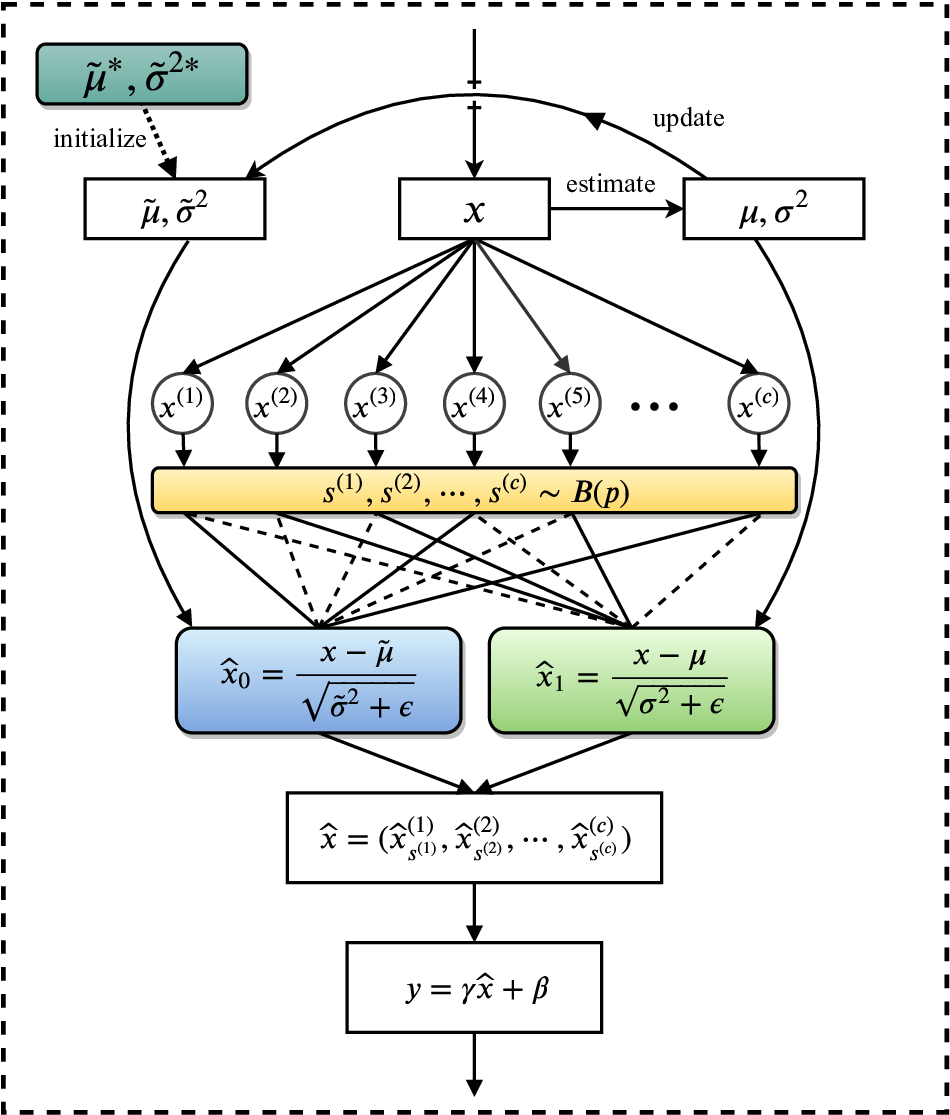
\includegraphics[width=\linewidth]{figures/绪论/arch.png}
    \caption{研究框架图}
    \label{fig:research}
\end{figure}

本文的主要创新点以及贡献如下:
\begin{itemize}
    \item 本文设计了一种全新的标准化层——随机标准化层(Stochastic Normalization,StochNorm),该标准化层超参数较少且结构简洁,具有很好的通用性,能够高效快捷地和现有的深度神经网络结构以及模型微调方法相结合。
    \item 本文针对模型微调场景,在多个细粒度图像分类数据集上使用带有StochNorm的深度神经网络进行训练,相较于传统的模型微调方法取得了明显的提升,并且能够很好地和这些方法进行结合,进一步提升效果。该部分算法研究成果发表在了机器学习顶级会议\textbf{NeurIPS-2019}(CCF-A,清华A类)上。
    \item 本文针对医疗影像诊断和金风风速预测两个实际场景,在基线深度神经网络结构中加入了StochNorm技术,均取得了一定的效果提升;
    \item 本文借助迁移学习算法库(Transfer Learning Library)的平台对StochNorm算法进行了集成与复现,取得了与本文实验部分一致的提升效果,提供了快捷调用的API接口。
\end{itemize}

\section{文章结构安排}
本文共计5个章节,主要内容安排如下:

第1章为绪论,主要介绍了本文的选题背景与意义,介绍了主要针对的两个场景,概括了本文的创新点和主要贡献。

第2章为相关工作介绍,介绍了模型微调领域和标准化层领域的发展历程和最新工作。

第3章主要介绍了本文提出的随机标准化层的算法细节,并在多个细粒度分类数据集上设计了实验,验证了该算法的性能。

第4章展示了StochNorm在实际场景中的应用,在医疗影像诊断和金风风速预测两个场景验证了该算法的有效性,并在迁移学习算法库中进行了集成,提供了快捷调用的API。

第5章对本文的工作进行了总结,并对未来工作进行了展望。
